%
% FROM OPEN GRAPHS TO OPEN OBJECTS
% Section
% V1
%

% --- comment out when compiling ---
%
%	REWRITING OPEN GRAPHS
%	preamble
%	v1

%  packages

\usepackage{amsfonts, amsthm, amssymb, amsmath, stmaryrd, etoolbox}
\usepackage{mathtools}
\usepackage{graphicx,caption,subcaption}
\usepackage{todonotes}
\usepackage{xcolor}
\usepackage{url}
\usepackage[inline]{enumitem}
	\setlist{itemsep=0em, topsep=0em, parsep=0em}
	\setlist[enumerate]{label=(\alph*)}
\usepackage[]{hyperref}
	\definecolor{hyperrefcolor}{rgb}{0,0,0.7}
	\hypersetup{colorlinks,linkcolor={hyperrefcolor},citecolor={hyperrefcolor},urlcolor={hyperrefcolor}}
\usepackage{tikz}
	\usetikzlibrary{matrix,arrows,shapes,decorations.markings,decorations.pathreplacing}
\usepackage[numbers]{natbib}
\usepackage{doi}

%
% commands
%

\newcommand{\RR}{\mathbb{R}}
\newcommand{\ZZ}{\mathbb{Z}}
\newcommand{\NN}{\mathbb{N}}
\newcommand{\QQ}{\mathbb{Q}}
\newcommand{\CC}{\mathbb{C}}
\newcommand{\DD}{\mathbb{D}}
\newcommand{\MM}{\mathbb{M}}
\renewcommand{\epsilon}{\varepsilon}

\newcommand{\defn}[1]{\textbf{#1}}
\newcommand{\op}[1]{\operatorname{#1}}
\newcommand{\cat}[1]{\mathbf{#1}}
\newcommand{\dblcat}[1]{\mathbb{#1}}
\renewcommand{\t}[1]{\text{#1}}

\newcommand{\from}{\colon}
\newcommand{\xto}[1]{\xrightarrow{#1}}
\newcommand{\sm}{\smallsetminus}
\newcommand{\tospan}{\xrightarrow{\mathit{sp}}}
\newcommand{\tocospan}{\xrightarrow{\mathit{csp}}}
\newcommand{\diagram}[1]{\raisebox{-0.5\height}{\includegraphics{#1}}}

\newcommand{\bispmap}[1]{\mathbf{Sp(#1)}}
\newcommand{\dblspmap}[1]{\mathbb{S}\mathbf{p(#1)}}
\newcommand{\bicspmap}[1]{\mathbf{Csp(#1)}}
\newcommand{\dblcspmap}[1]{\mathbb{C}\mathbf{sp(#1)}}
\newcommand{\bispsp}[1]{\mathbf{Sp(Sp(#1))}}
\newcommand{\dblspsp}[1]{\mathbb{S}\mathbf{p(Sp(#1))}}
\newcommand{\bicspcsp}[1]{\mathbf{Csp(Csp(#1))}}
\newcommand{\dblcspcsp}[1]{\mathbb{C}\mathbf{sp(Csp(#1))}}
\newcommand{\bimonspcsp}[1]{\mathbf{MonicSp(Csp(#1))}}
\newcommand{\dblmonspcsp}[1]{\mathbb{M}\mathbf{onicSp(Csp(#1))}}
\newcommand{\biepiccspsp}[1]{\mathbf{EpicCsp(Sp(#1))}}
\newcommand{\dblepiccspsp}[1]{\mathbb{E}\mathbf{picCsp(Sp(#1))}}
\newcommand{\spcsp}[1]{\mathbf{Sp(Csp(#1))}}
\newcommand{\dblspcsp}[1]{\mathbb{S}\mathbf{p(Csp(#1))}}

\newcommand{\LspanD}{ L \t{-} \operatorname{Span} ( \mathbf{D} ) }
\newcommand{\LopenD}{ L \t{-} \operatorname{Open} }
\newcommand{\LrewriteD}{ L \t{-} \operatorname{Rewrite} }

%
% math operators
%

\DeclareMathOperator{\Hom}{Hom}
\DeclareMathOperator{\id}{id}
\DeclareMathOperator{\ob}{Ob}
\DeclareMathOperator{\arr}{arr}
\DeclareMathOperator{\im}{im}
\DeclareMathOperator{\Aut}{Aut}
\DeclareMathOperator{\Bij}{Bij}
\DeclareMathOperator{\Sub}{Sub}
\DeclareMathOperator{\colim}{colim}

%
% envirnments and counters
%

\newtheorem{thm}{Theorem}[section]
\newtheorem{lem}[thm]{Lemma}
\newtheorem{prop}[thm]{Proposition}
\newtheorem{cor}[thm]{Corollary}

\theoremstyle{remark}
	\newtheorem{remark}[thm]{Remark}
	\newtheorem{notation}[thm]{Notation}

\theoremstyle{definition}
	\newtheorem{ex}[thm]{Example} 
	\newtheorem{df}[thm]{Definition}

% \setcounter{tocdepth}{1} % Sets depth for table of contents. 

%
% tikz types
%

\tikzset{->-/.style={decoration={%
			markings,
			mark=at position .5 with {\arrow{>}}},postaction={decorate}}
}
\tikzset{->-pos/.style={decoration={%
			markings,
			mark=at position #1 with {\arrow{>}}},postaction={decorate}}
}
\tikzset{->-/.style={decoration={%
			markings,
			mark=at position .5 with {\arrow{>}}},postaction={decorate}}
}
\tikzset{->-pos/.style={decoration={%
			markings,
			mark=at position #1 with {\arrow{>}}},postaction={decorate}}
}
 % input preamble
\bibliography{3--RewriteOpenGraphs--Bibliography}	

\section{From open graphs to open objects} % section title

In the previous section,
we defined an open graph,
a important object of study
in network theory.
But for many networks,
open graphs are too structure poor.
They just don't capture all of
the information that a network may have.
And so, we need to generalize open graphs
to open objects.

Given categories $\cat{C}$ and $\cat{D}$
with coproducts together with a full and faithful
functor $L \from \cat{C} \to \cat{D}$
preserving coproducts, we define an
\defn{$L$-open object of $\cat{D}$} to be a cospan
of the form $ L ( x ) \to y \gets L ( z ) $.
When there is little chance for confusion,
we will merely use the term `open object'.

A morphism of open objects is a triple
$ (f,g,h) $ that fits into a commuting diagram
\[
	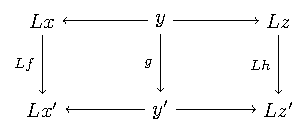
\includegraphics[]{InclGrphx--Diagram--OpenObjectArrow}
\]

Much has been written about
graph rewriting theory. 
Here, we intend to extend
these results to open graphs,
and further, to open objects.
Lack and Sobocinski 
\todo{
	citation
}
have shown that topoi
admit a nice rewriting theory.
Hence, we prove the following
theorems. 
  











